\chapter{Measurements}
\label{chap:measurement}

In order to be able to validate the results obtained from the finite element simulation (see \cref{chap:results}), specific measurements have been carried out.
In this chapter, the acoustic power measurement of the sound source and the outer pressure field measurement around the car body are presented.
The obtained sound power spectrum of the omnidirectional loudspeaker provides simulation input for the finite element analysis in section \ref{section:boundary_conditions}.
Furthermore, the measurement results of outer pressure field serve as validation for the finite element model in \cref{chap:results}.

\section{Characterisation of sound source}
\label{section:SWL_measurement}

Two important characteristics of a sound source are directivity and sound power. For the validation measurement, a dodecahedron loudspeaker of type Brüel \& Kjaer 4292-L is used as excitation, which can be treated as an omnidirectional sound source.
Hence, only the sound power emitted by the loudspeaker is of interest.
In the following, the acoustic power spectrum of the sound source is measured following ISO 9614-2 \cite{din19969614}.

\subsection*{Measurement setup}

In \cref{fig:soundpowersetup} the measurement setup for the determination of sound power levels is shown.
The omnidirectional loudspeaker was placed on a reflective concrete floor and was enveloped by a 1m x 1m x 1m reference box.
The loudspeaker was driven by a reference amplifier with pink noise as an input signal (\cref{fig:signalgenerator}).
In order to reduce fluctuations in output power, the amplifier was switched on and warmed up for at least 20 minutes before the start of the measurement.
% weniger Absätze verbessern den Lesefluss.
% Ein Absattz sollte zumindest 3 Sätze haben
The measurement was carried out according to the ISO 9614-2 standard, in which the sound power is determined from intensity measurement over measurement surfaces.
This method has the advantage that room reflections and any sound sources outside of the reference box do not influence the measurement result.
The intensity measurements were done using the Brüel \& Kjaer sound intensity probe kit type 3654, which includes a pair of microphones that are placed face to face with each other, separated by a spacer.

% Absatz "2 microphone Intensity measurement"
This method of intensity measurement is also called two-microphone method or $p-p$ method.
% jeder Satz in einer eigenen Zeile gibt besser git-diffs ...
Instead of direct measurement, the particle velocity is obtained by a finite-difference approximation to the pressure gradient \cite{jocobsen_2005}\cite{moschioni_2008}.
% willst du den ganzen Ansatz zitieren? Dann ist [ref] nach . richtig.
% Ansonsten wäre dies ein Anbsatz mit "2 microphone Intensity measurement" als Thema
In the following, the basic concept of sound power measurement using the two-microphone method is shown. The relation between particle velocity $\boldsymbol{u_a}$ and the acoustic pressure $p_a$ is described by the Euler equation of motion
\begin{equation}
    \rho_0 \frac{\partial \boldsymbol{u_a}}{\partial t} = -\nabla p_a \text{.} \label{eq:euler_equatioin}
\end{equation}
In the intensity measurement using the two-microphone method (\cref{fig:scanningmethod}), the intensity probe is moved over the measurement surface with a constant speed and is kept perpendicular to the scanned area so that only the normal component of the particle velocity is captured. Furthermore, the normal component of the pressure gradient in \cref{eq:euler_equatioin} is approximated by the finite difference of the measured pressures. \Cref{eq:euler_equatioin} for the normal component then reads as
\begin{equation}
	\rho_0\frac{\partial(\boldsymbol{u_a} \cdot \boldsymbol{n})}{\partial t} = -\nabla p_a \cdot \boldsymbol{n} \approx -\frac{p_2 - p_1}{\Delta r}\text{,}
\end{equation}
with $p_1$ and $p_2$ being the measured pressure of the microphone closer and further from the incident sound wave, respectively, $\Delta r$ being the thickness of the spacer and $\boldsymbol{n}$ the unit normal vector of the measurement surface. Hence, the normal particle velocity $u_n$ can be expressed as
\begin{equation}
   u_n = \boldsymbol{u_a} \cdot \boldsymbol{n} = \int\frac{(p_1 - p_2)}{\rho_0 \Delta r}\dif t \text{.}
\end{equation}
The normal component of the sound intensity is then obtained by the product of the approximated particle velocity and the mean of the measured pressures
\begin{equation}
    I_n = \boldsymbol{I_a} \cdot \boldsymbol{n} = p_a u_n = \frac{p_1 + p_2}{2} \int\frac{(p_1 - p_2)}{\rho_0 \Delta r}\dif t\text{.}
\end{equation}
Each partial measurement surface is scanned twice, using a vertical and a horizontal scan path, respectively. The obtained result is the spatially averaged intensity $\langle I_{n}\rangle$. The sound power of a single measurement surface is then given by the product of the spatial average intensity and the surface area by
\begin{equation}
    W_i = \langle I_{n\text{,}i}\rangle S_i\,.
\end{equation}
The total sound power of the enclosed sound source is then given by the sum of the sound power of each measurement surface and reads as
\begin{equation}
    W_{total} = \sum_{i = 1}^{N} W_i\,.
\end{equation}

% Beispiel für eine Grafik
\begin{figure}[H]
\begin{center}
\includegraphics[width=12cm]{fig/Sound_power_measurement.png}
\caption{Setup for sound power measurement.}
\label{fig:soundpowersetup}
\end{center}
\end{figure}

\begin{figure}[H]
     \centering
     \begin{subfigure}[b]{0.5\textwidth}
         \centering
         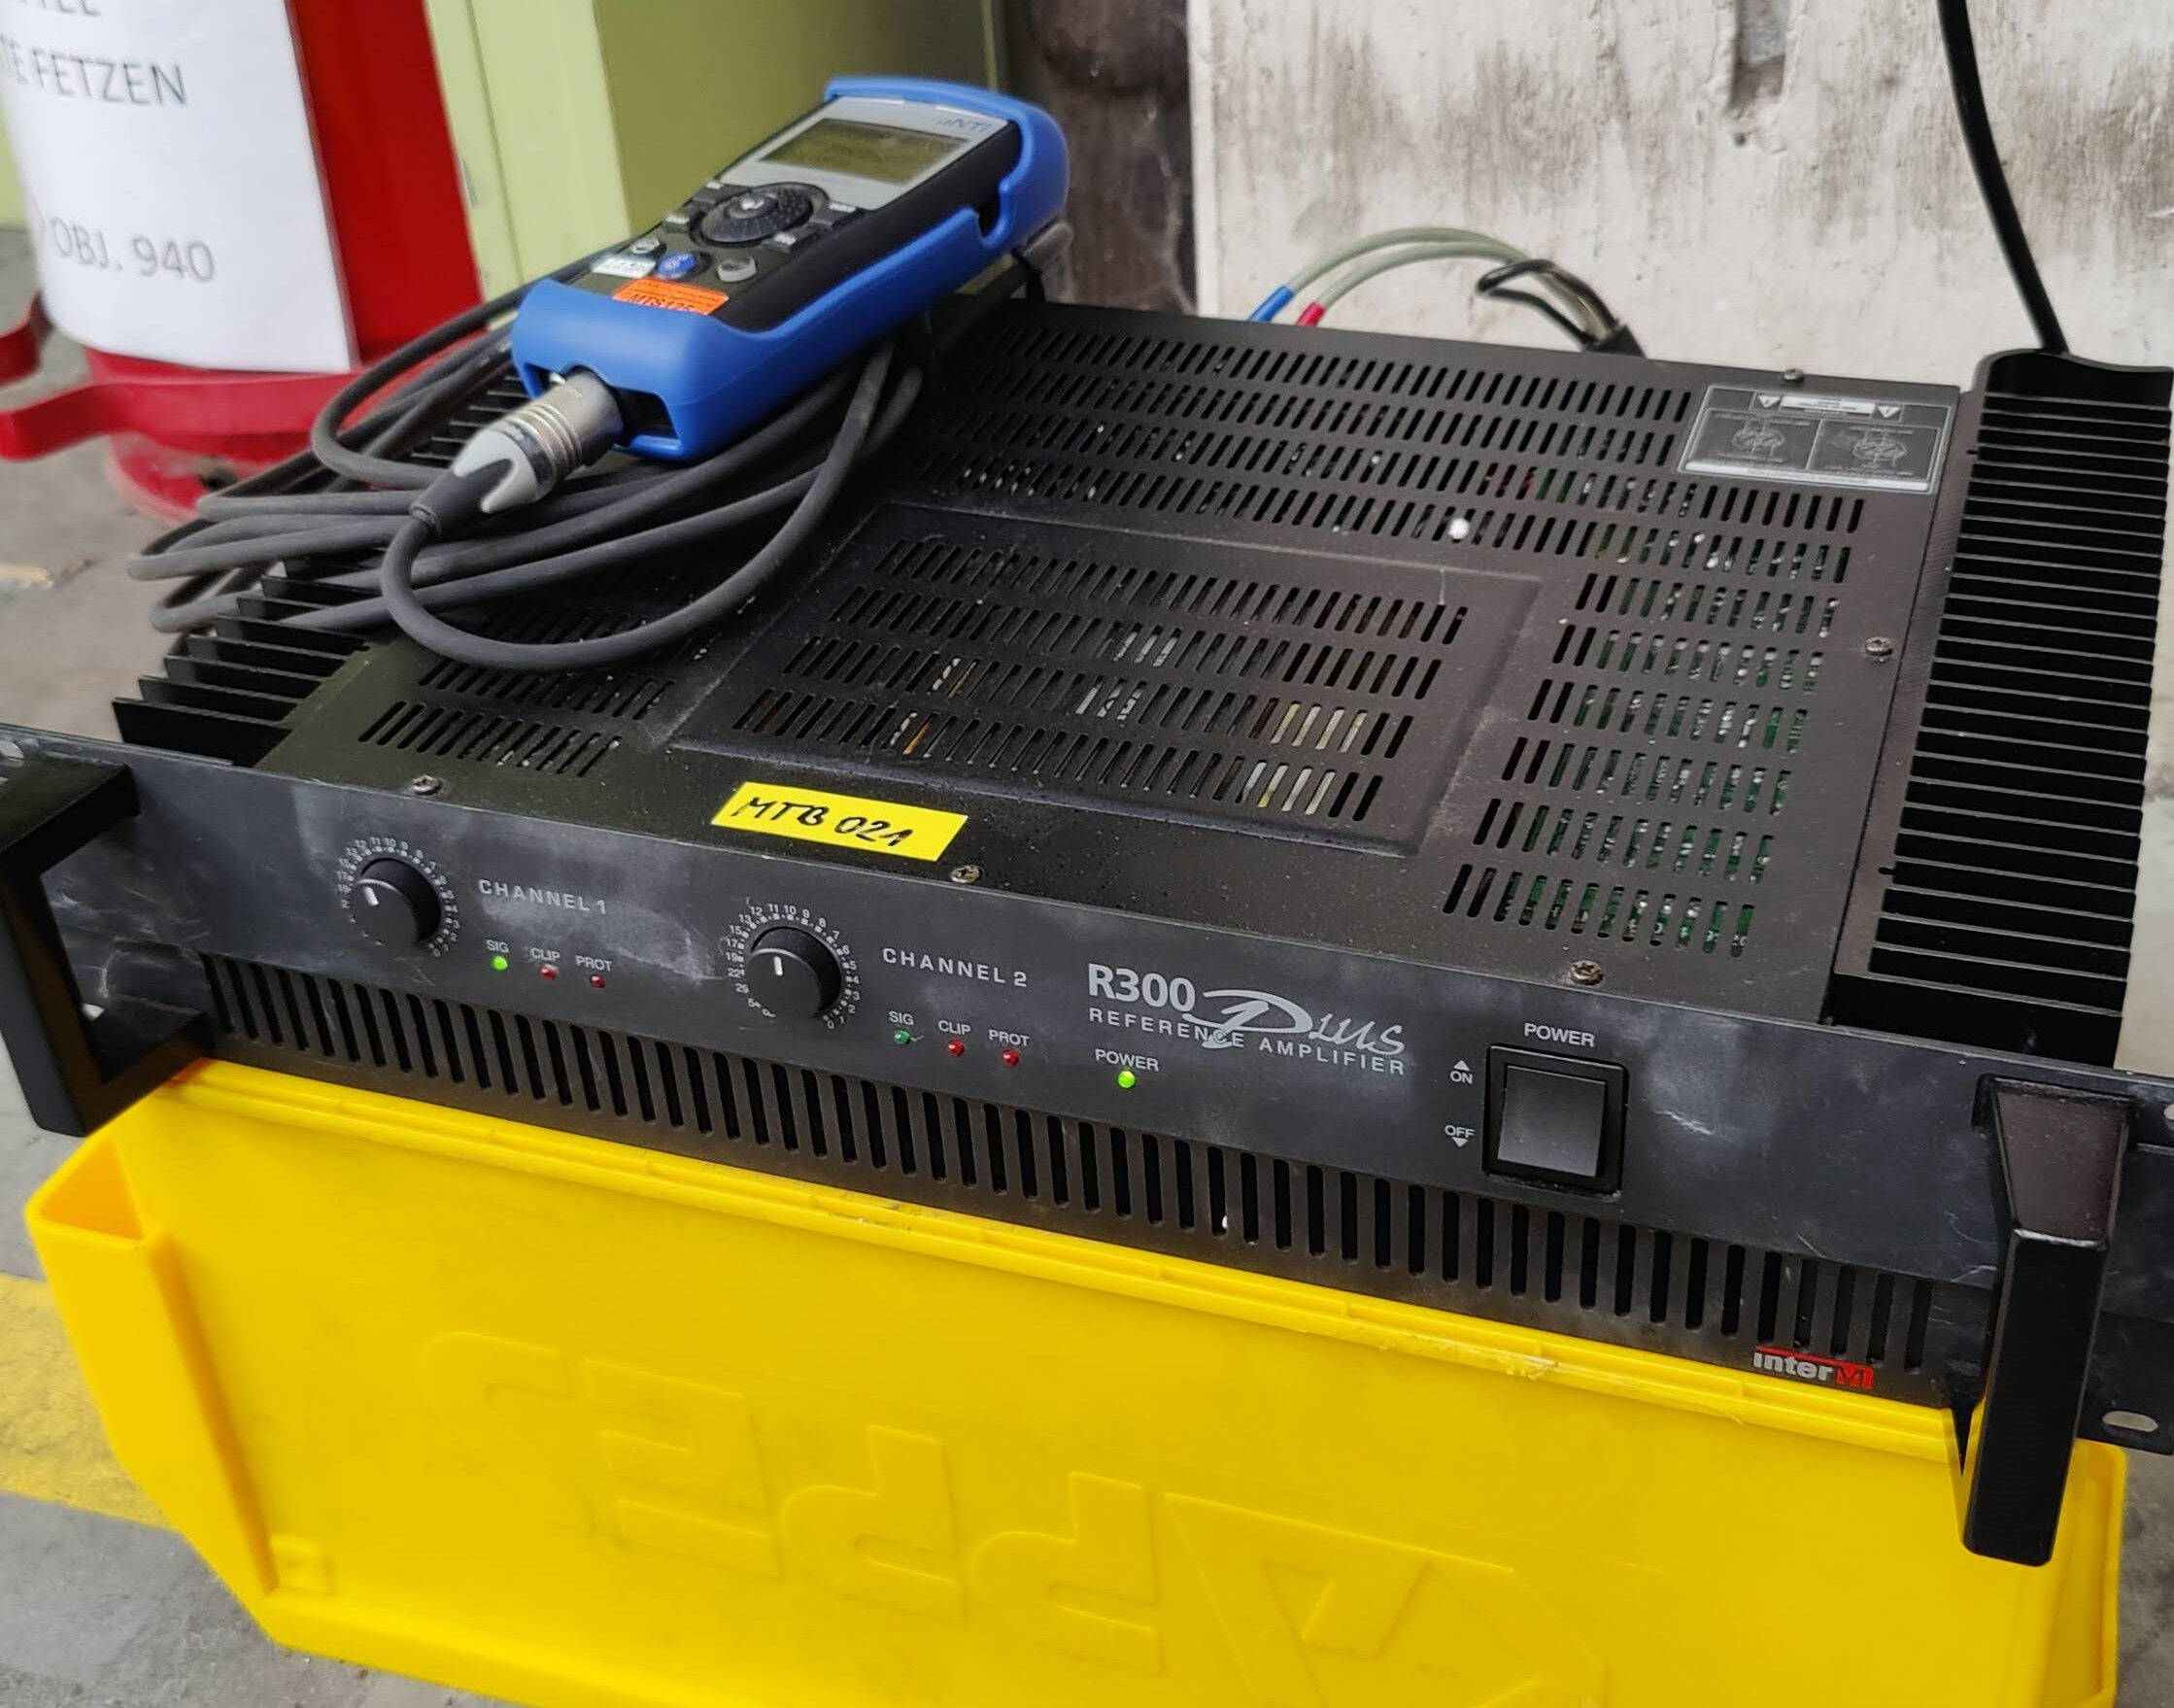
\includegraphics[width=\textwidth]{fig/amplifier_and_signal_generator.jpg}
         \caption{Inter-M R300 Plus reference amplifier}
     \end{subfigure}
     \hspace{0.1\textwidth}
     %\hfill
     \begin{subfigure}[b]{0.3\textwidth}
         \centering
         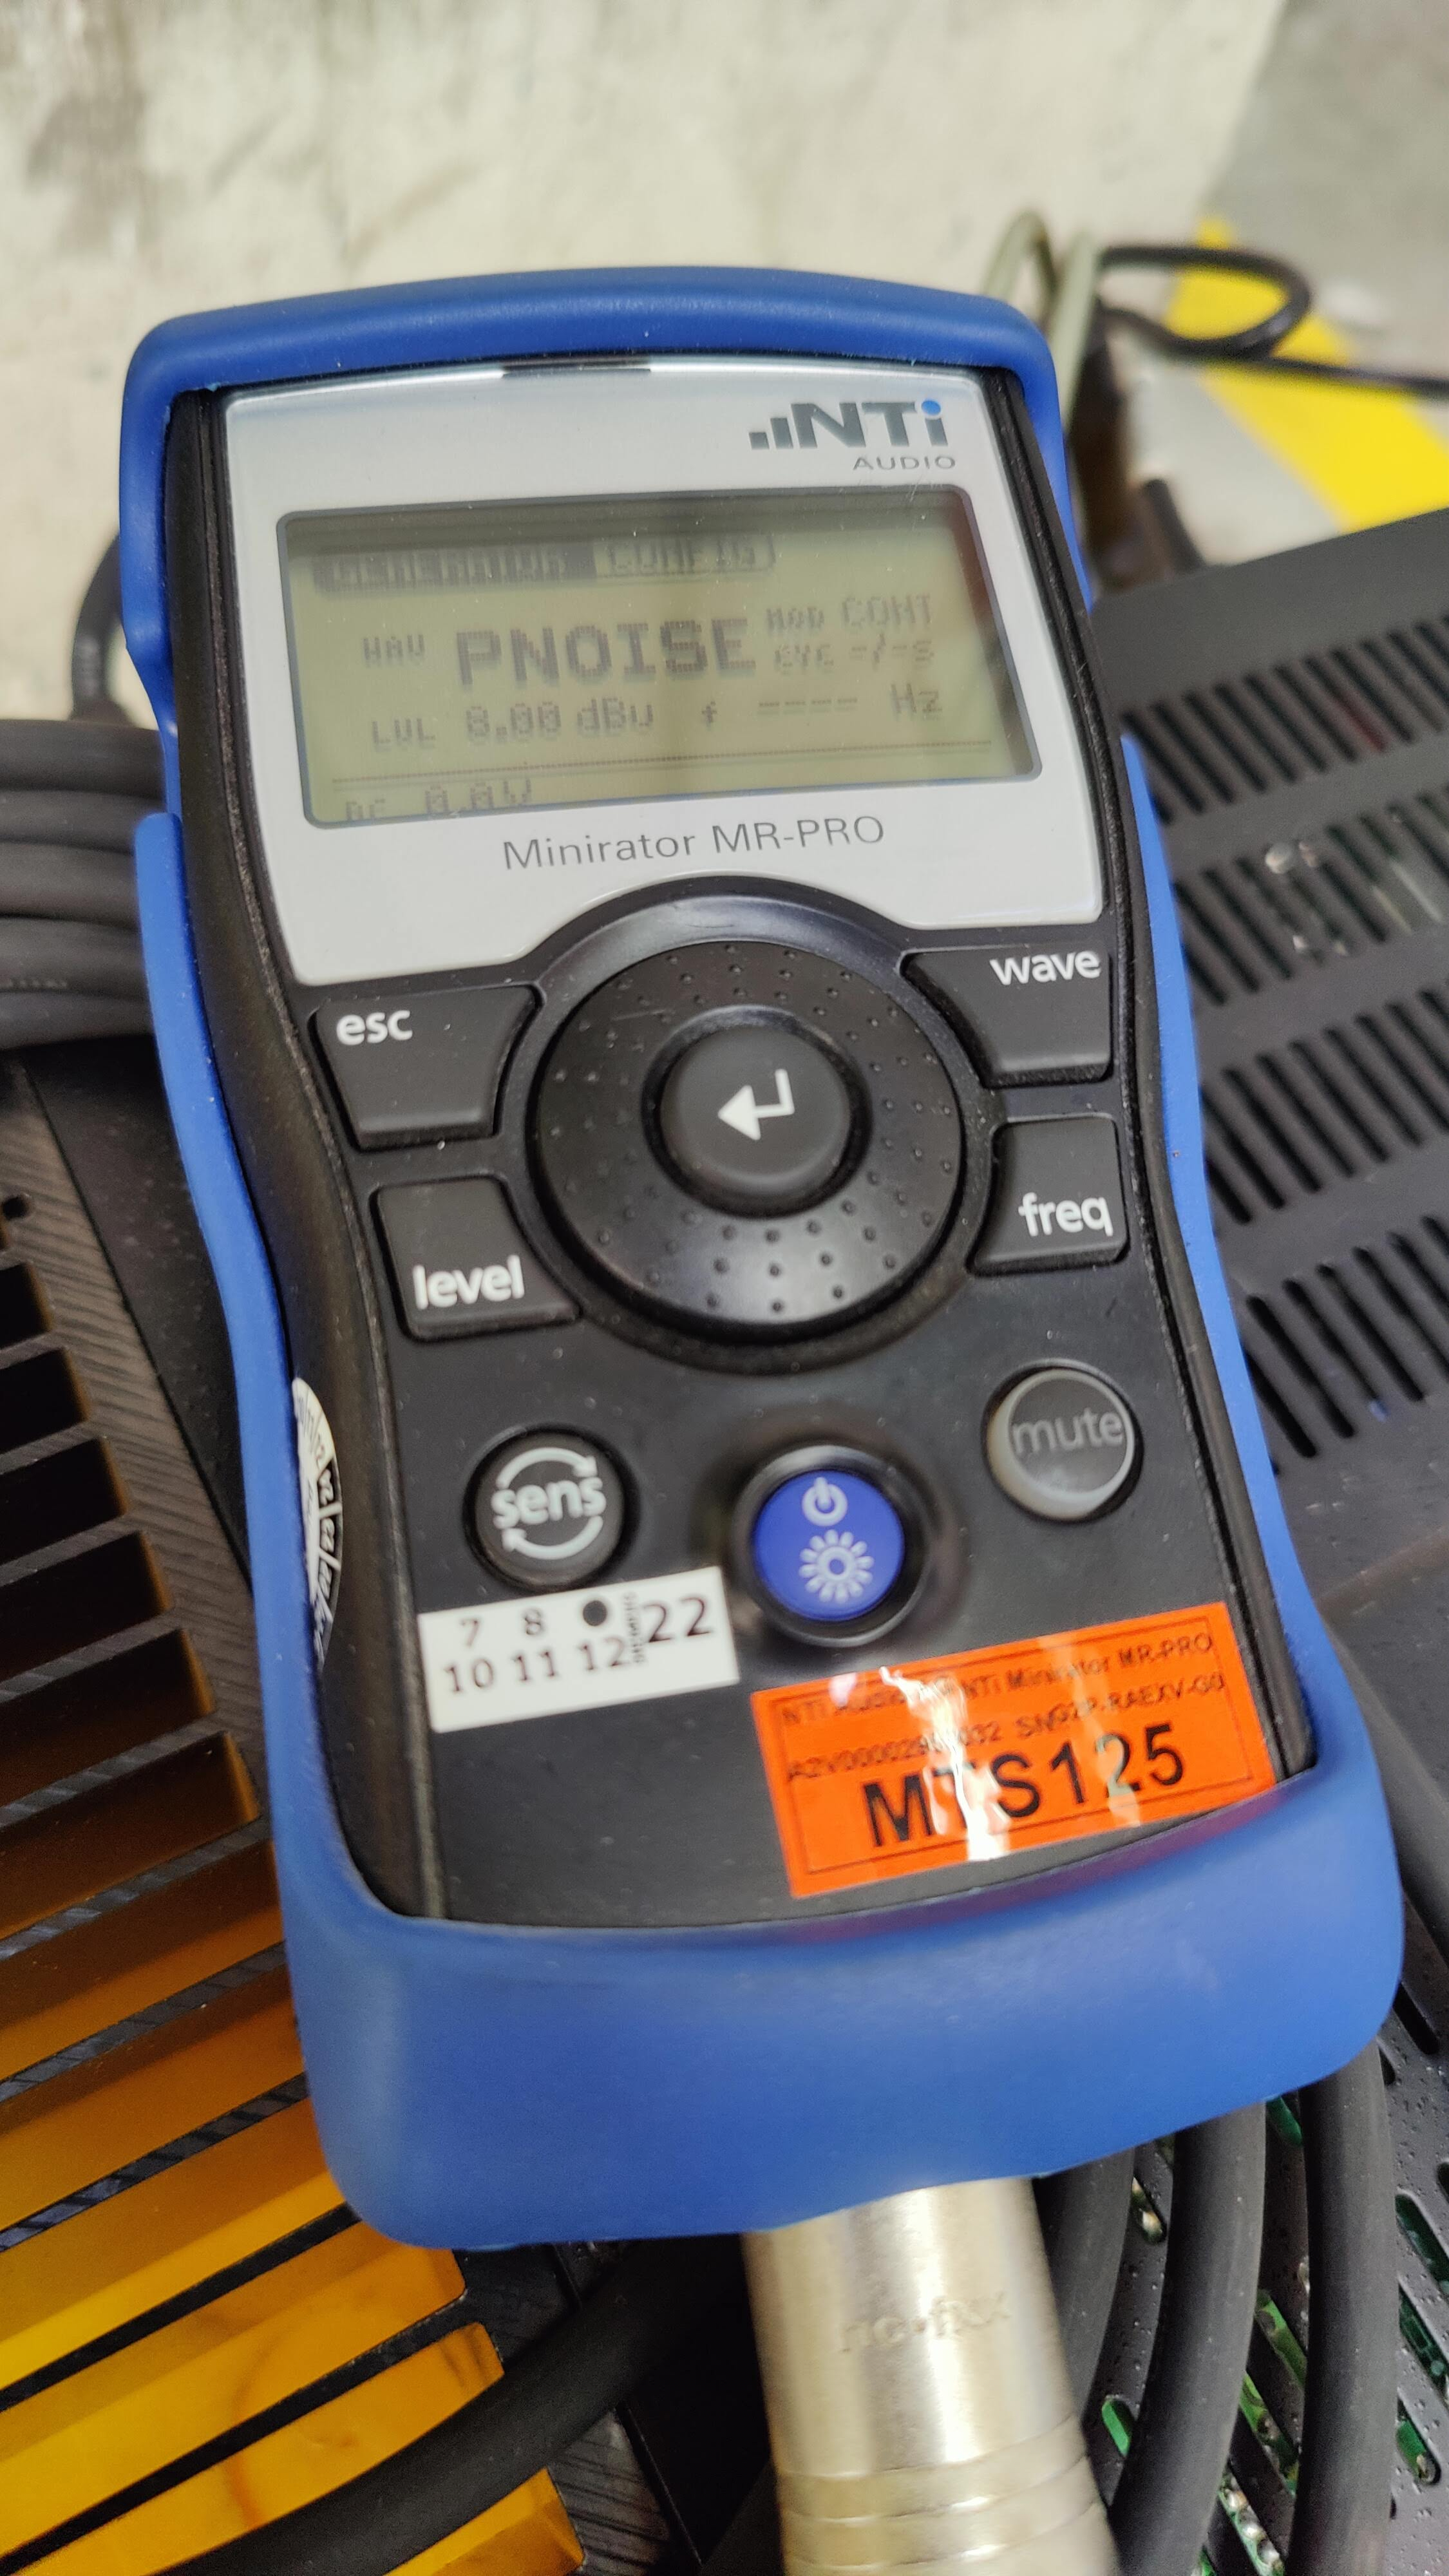
\includegraphics[width=\textwidth]{fig/signal_generator.jpg}
         \caption{NTI Minirator MR-PRO}
     \end{subfigure}
        \caption{Signal generator and amplifier.}
        \label{fig:signalgenerator}
\end{figure}

\begin{figure}[H]
\begin{center}
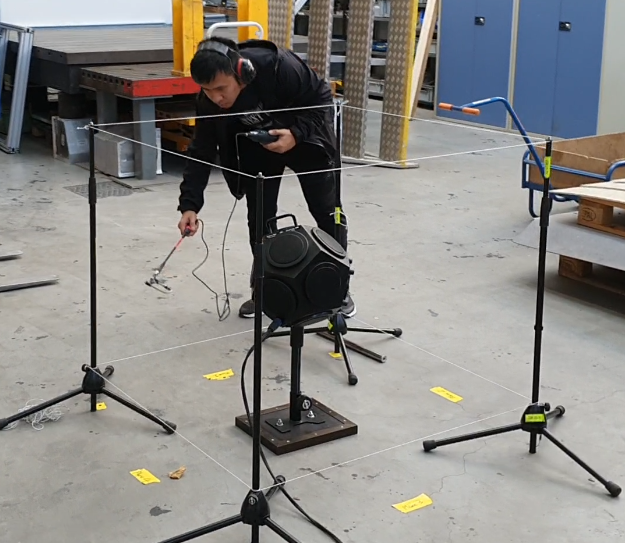
\includegraphics[width=12cm]{fig/Sound_power_measurement_2.png}
\caption{Intensity measurement using the two-microphone method according to ISO 9614-2 \cite{din19969614}.}
\label{fig:scanningmethod}
\end{center}
\end{figure}

\subsection*{Measurement results}

The measurement is post-processed using the Brüel \& Kjaer type 2270 hand-held analyzer and the result is shown in one-third octave band spectra. \Cref{fig:SWL} shows the measured non-weighted (Z-weighting) sound power level (SWL ref \SI{1}{\pico\watt}) from \SIrange{100}{2000}{\hertz}. The measurement was carried out twice, and the deviation of both measurements was  within \SI{0.3}{\dB} in total power. For the finite element simulation, the averaged value of both measurements as shown in \cref{fig:average_SWL} was used.

\begin{figure}[H]
     \centering
     \begin{subfigure}[b]{0.9\textwidth}
         \centering
         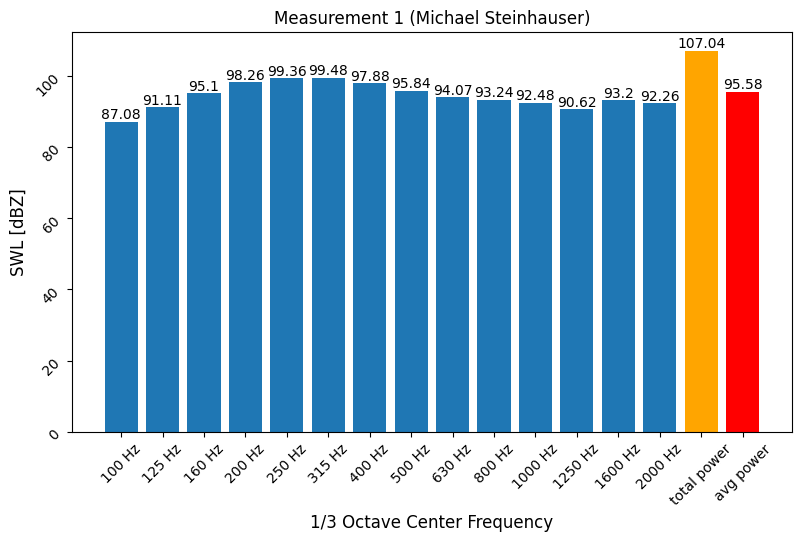
\includegraphics[width=\linewidth]{fig/SWL_1.png}
         \caption{Measurement series 1}
     \end{subfigure}
     \par\bigskip
     %\hspace{0.1\textwidth}
     %\hfill
     \begin{subfigure}[b]{0.9\textwidth}
         \centering
         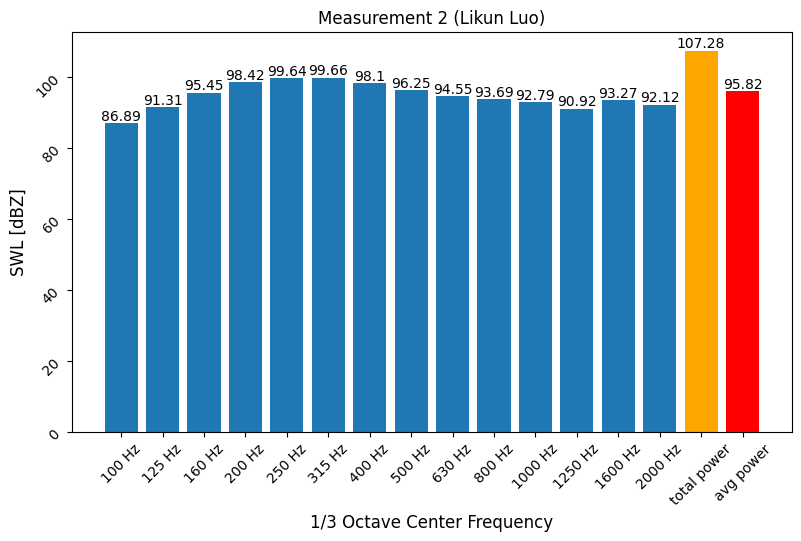
\includegraphics[width=\linewidth]{fig/SWL_2.png}
         \caption{Measurement series 2}
     \end{subfigure}
\end{figure}

\begin{figure}[H]\ContinuedFloat
     \centering
     \begin{subfigure}[b]{0.9\textwidth}
         \centering
         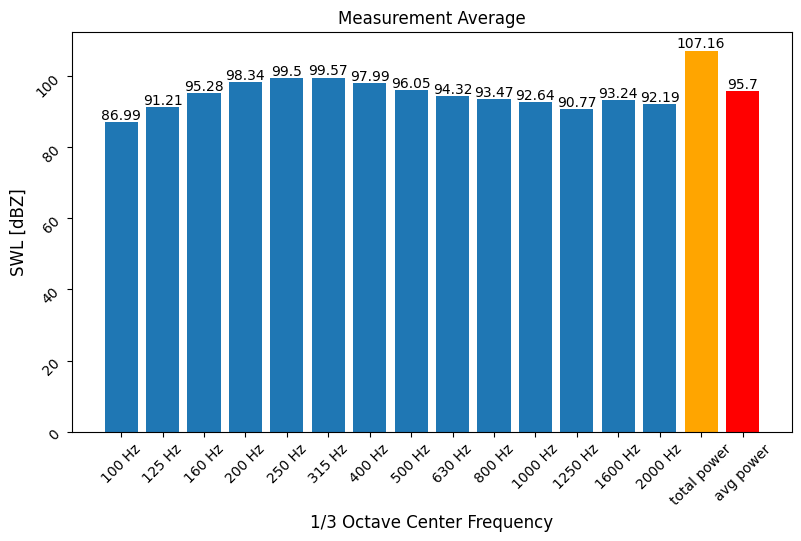
\includegraphics[width=\linewidth]{fig/SWL_average.png}
         \caption{Averaged value of both measurement series}
         \label{fig:average_SWL}
     \end{subfigure}
     
        \caption{Sound power spectra in 1/3-octave bands, SWL in \SI{}{\dB} ref \SI{1}{\pico\watt}.}
        \label{fig:SWL}
\end{figure}


\section{Pressure field measurement on a standing metro train}
\label{sec:pressure_field_measurement}

In this section, we describe the sound pressure measurements which were done on a standing UBX metro with controlled excitation.
The reason to perform measurements under standstill conditions was to avoid the uncertainties introduced by the complex real sources (e.g. wheel-rail interaction) in dynamic conditions. With this approach, the quality of the finite element model can be better assessed.

\subsection*{Measurement setup}

The measurement was performed on October 4, 2022 at the company premises of Siemens Mobility Austria in 1110 Vienna. The measurement setup is shown in \cref{fig:outersetup}. \Cref{fig:ubxfrontview} shows the front car of the measurement vehicle of type Siemens U-Bahn Wien X. In order to approximate free field conditions as closely as possible, the measurement vehicle was parked in a relatively empty area of company premises to avoid environmental reflections as much as possible.

To evaluate the outer pressure field close to the car body, 10 pressure microphones were arranged in a line array order, allowing simultaneous measurement along the height direction. As shown in \cref{fig:ubxsideview}, the microphones were attached on a tripod at a distance of half a meter to each other, the position of the microphones started at 0.5 m and ended at 5 m above ground.

The acoustic excitation came from an omnidirectional loudspeaker with pink noise as an input signal, using identical settings as in the previous acoustic power measurement. The loudspeaker was placed beneath the car underframe in the empty space between the bogie axle and the wheel axle, at about 55 cm above the ground (see \cref{fig:loudspeakerposition}). Measurements have been performed with 2 different loudspeaker locations. One at the front of the bogie (Position A), and the other at the rear (Position B), as marked in \cref{fig:ubxsideview}. The aim was to evaluate the possible asymmetric effect caused by the anti-symmetric layout of the bogie components (e.g. brake discs), also it provides validation for the finite element model, which will exploit the symmetry using the image-source technique.

Due to the limited availability of the measurement vehicle, the measurement was concentrated on only one side of the vehicle, near the front bogie. In \cref{fig:microphoneposition}, all measurement positions of the microphone array are shown and labeled. Position a is the starting position of measurement, it lies on the centerline of the bogie frame, 10 cm away from the car body edge (see \cref{fig:position_a}). The full description of measurement positions is found in \cref{tab:measurement_positons}.

\begin{table}[H]
	\begin{tabular}{cc}
		\toprule
		Position  & Description                                                                     \\
		\midrule
		a              & on bogie centerline , 10 cm away from carbody edge                              \\
		b              & 50 cm out of bogie centerline in front direction, 10 cm away from carbody edge  \\
		c              & 100 cm out of bogie centerline in front direction, 10 cm away from carbody edge \\
		d              & 50 cm out of bogie centerline in rear direction, 10 cm away from carbody edge   \\
		e              & 100 cm out of bogie centerline in rear direction, 10 cm away from carbody edge  \\
		f              & on bogie centerline , 50 cm away from carbody edge                              \\
		g              & on bogie centerline , 100 cm away from carbody edge                             \\
		h              & on bogie centerline , 150 cm away from carbody edge                             \\ 
		i              & on bogie centerline , 200 cm away from carbody edge                             \\ 
		\bottomrule
	\end{tabular}
	\caption{Description of measurement positions.}
	\label{tab:measurement_positons}
\end{table}
\noindent At each measurement position, the multi-channel time-varing signal of the pressure field was captured by the Müller-BBM PAK MKII data acquisition system. The duration of a single measurement run was set to 15 seconds. The captured time signal will be post-processed using the provided Müller-BBM PAK software suit.

\begin{figure}[H]
     \centering
     \begin{subfigure}[b]{0.7\textwidth}
         \centering
         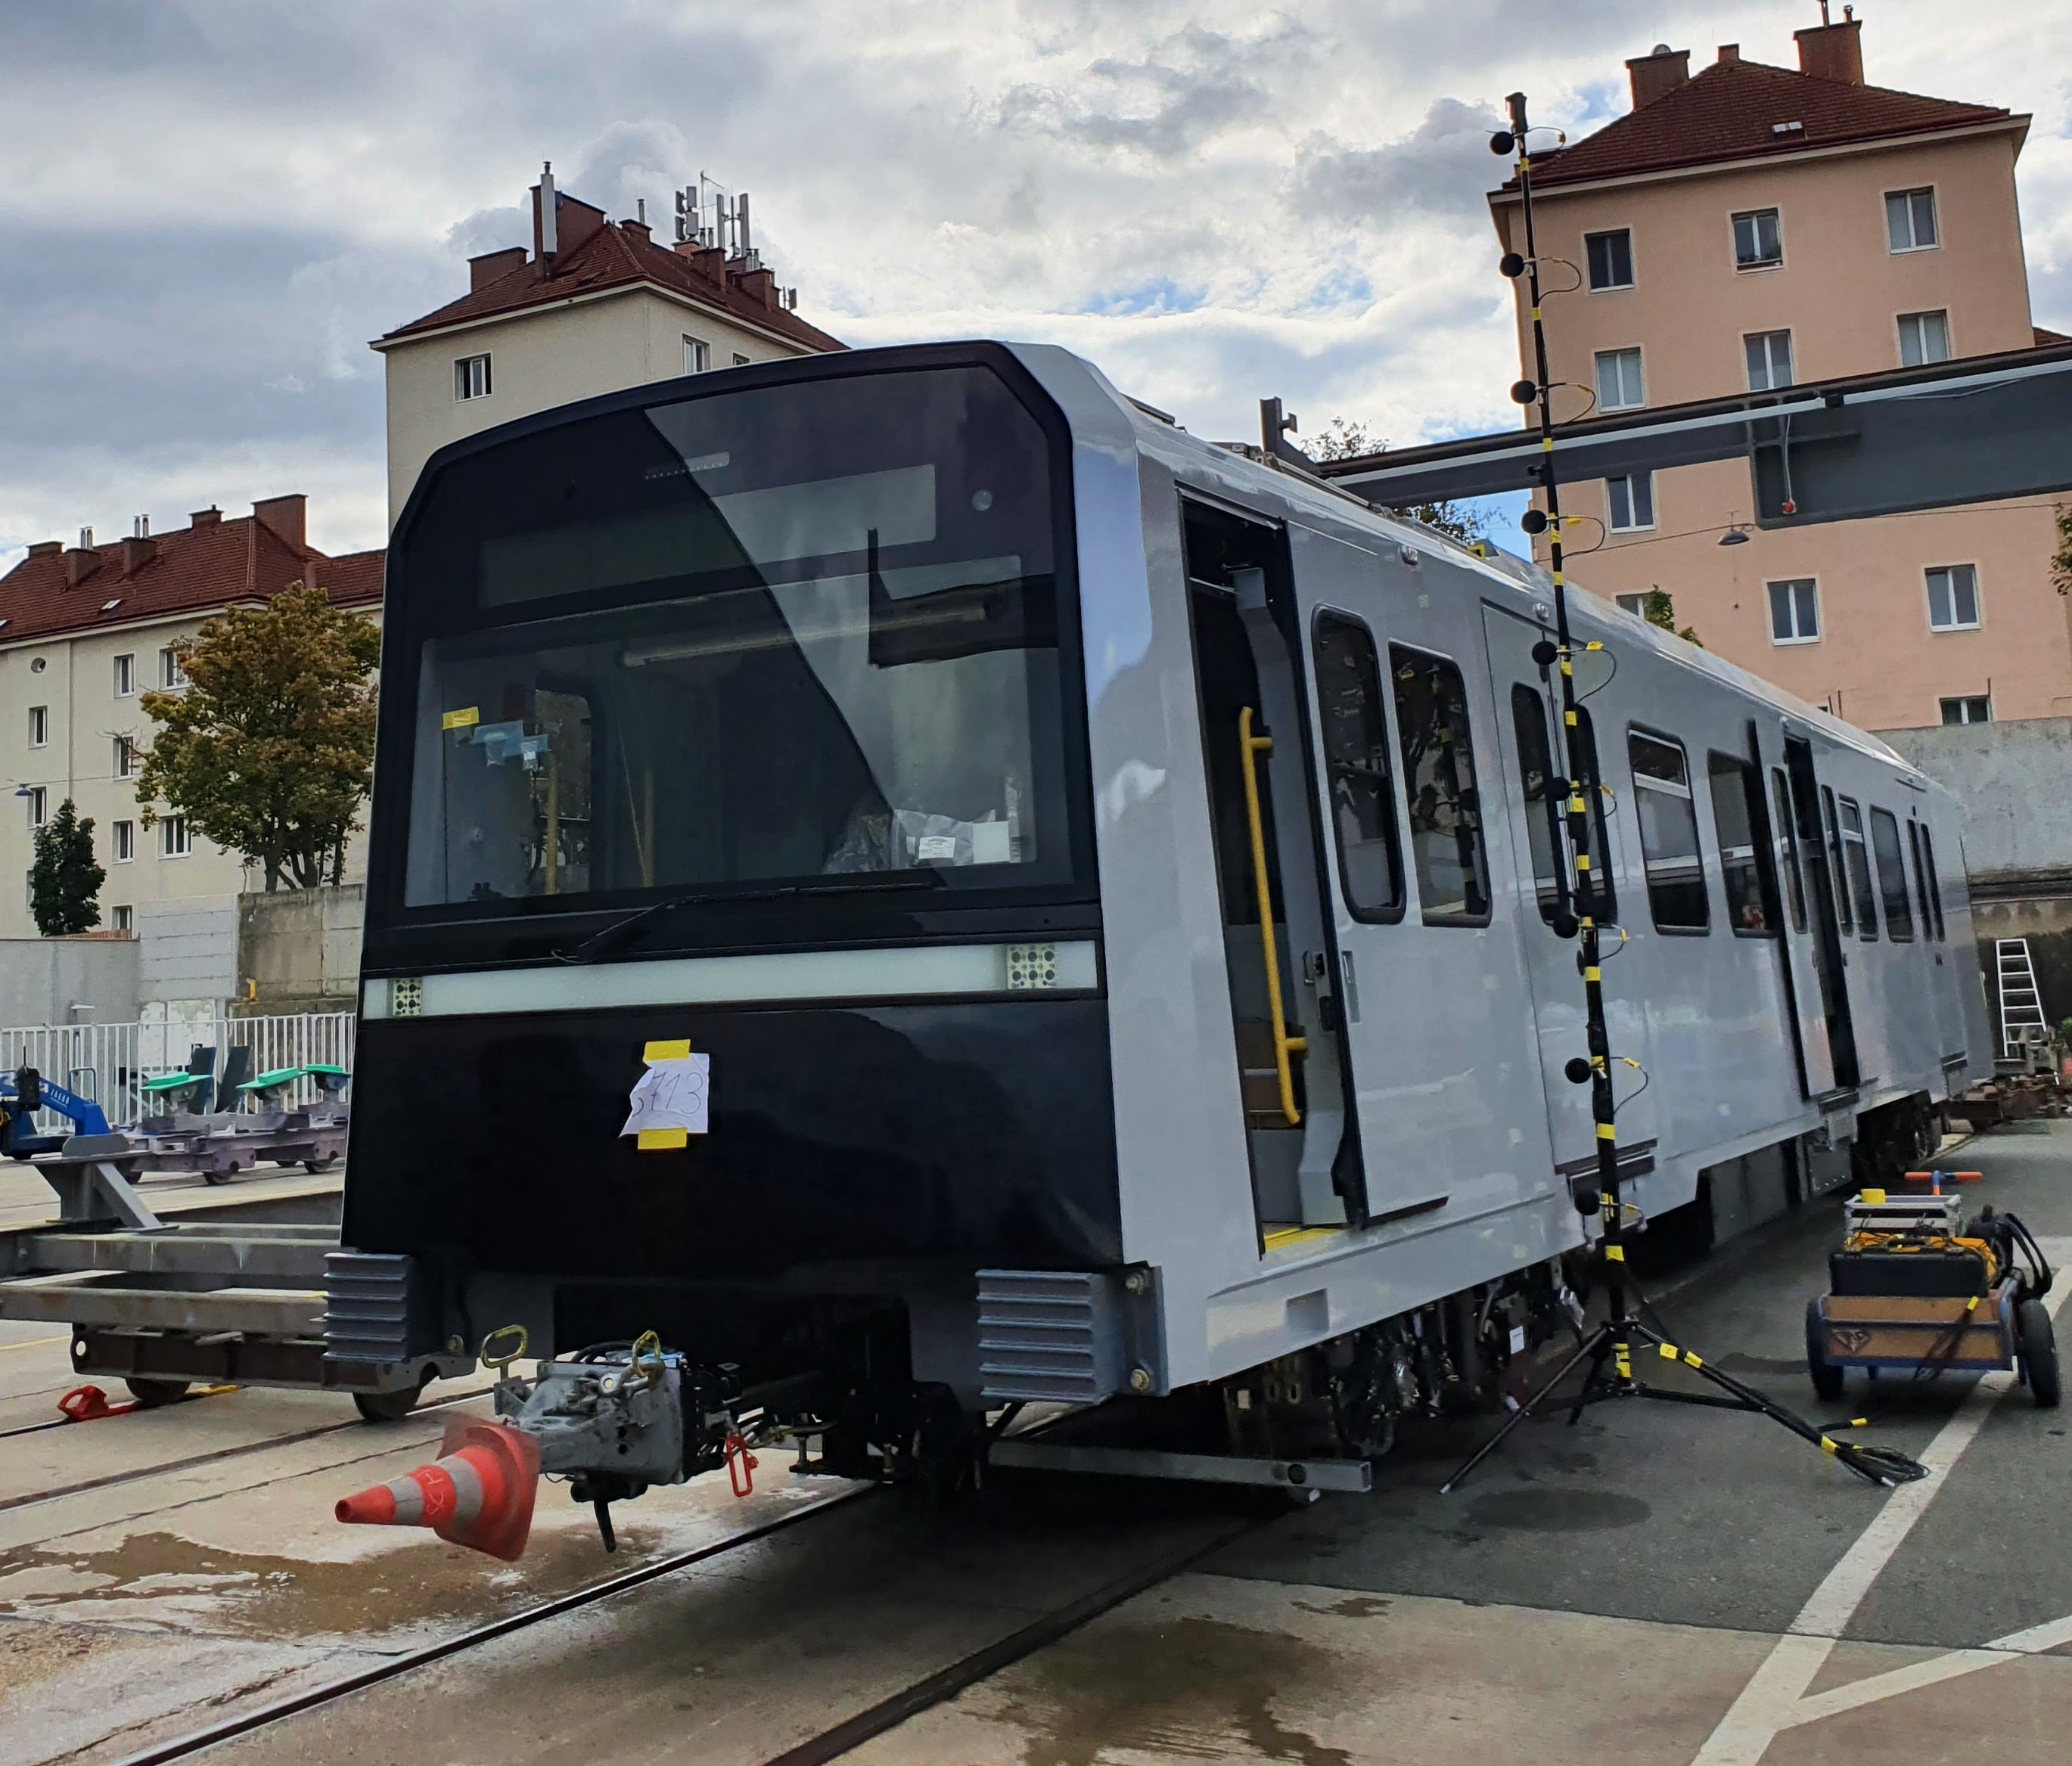
\includegraphics[width=\linewidth]{fig/Static_measurement_front_view.jpg}
         \caption{Front view}
         \label{fig:ubxfrontview}
     \end{subfigure}
     %\par\bigskip
     %\hspace{0.1\textwidth}
     %\hfill
\end{figure}

\begin{figure}[H]\ContinuedFloat
    \centering
    \begin{subfigure}[b]{\textwidth}
         \centering
         \includegraphics[width=\linewidth]{fig/Static_measurement_side_view.png}
         \caption{Side view}
         \label{fig:ubxsideview}
     \end{subfigure}
     \caption{Outer pressure field measurement setup.}
     \label{fig:outersetup}
\end{figure}

\begin{figure}[H]
     \centering
     \begin{subfigure}[b]{0.4\textwidth}
         \centering
         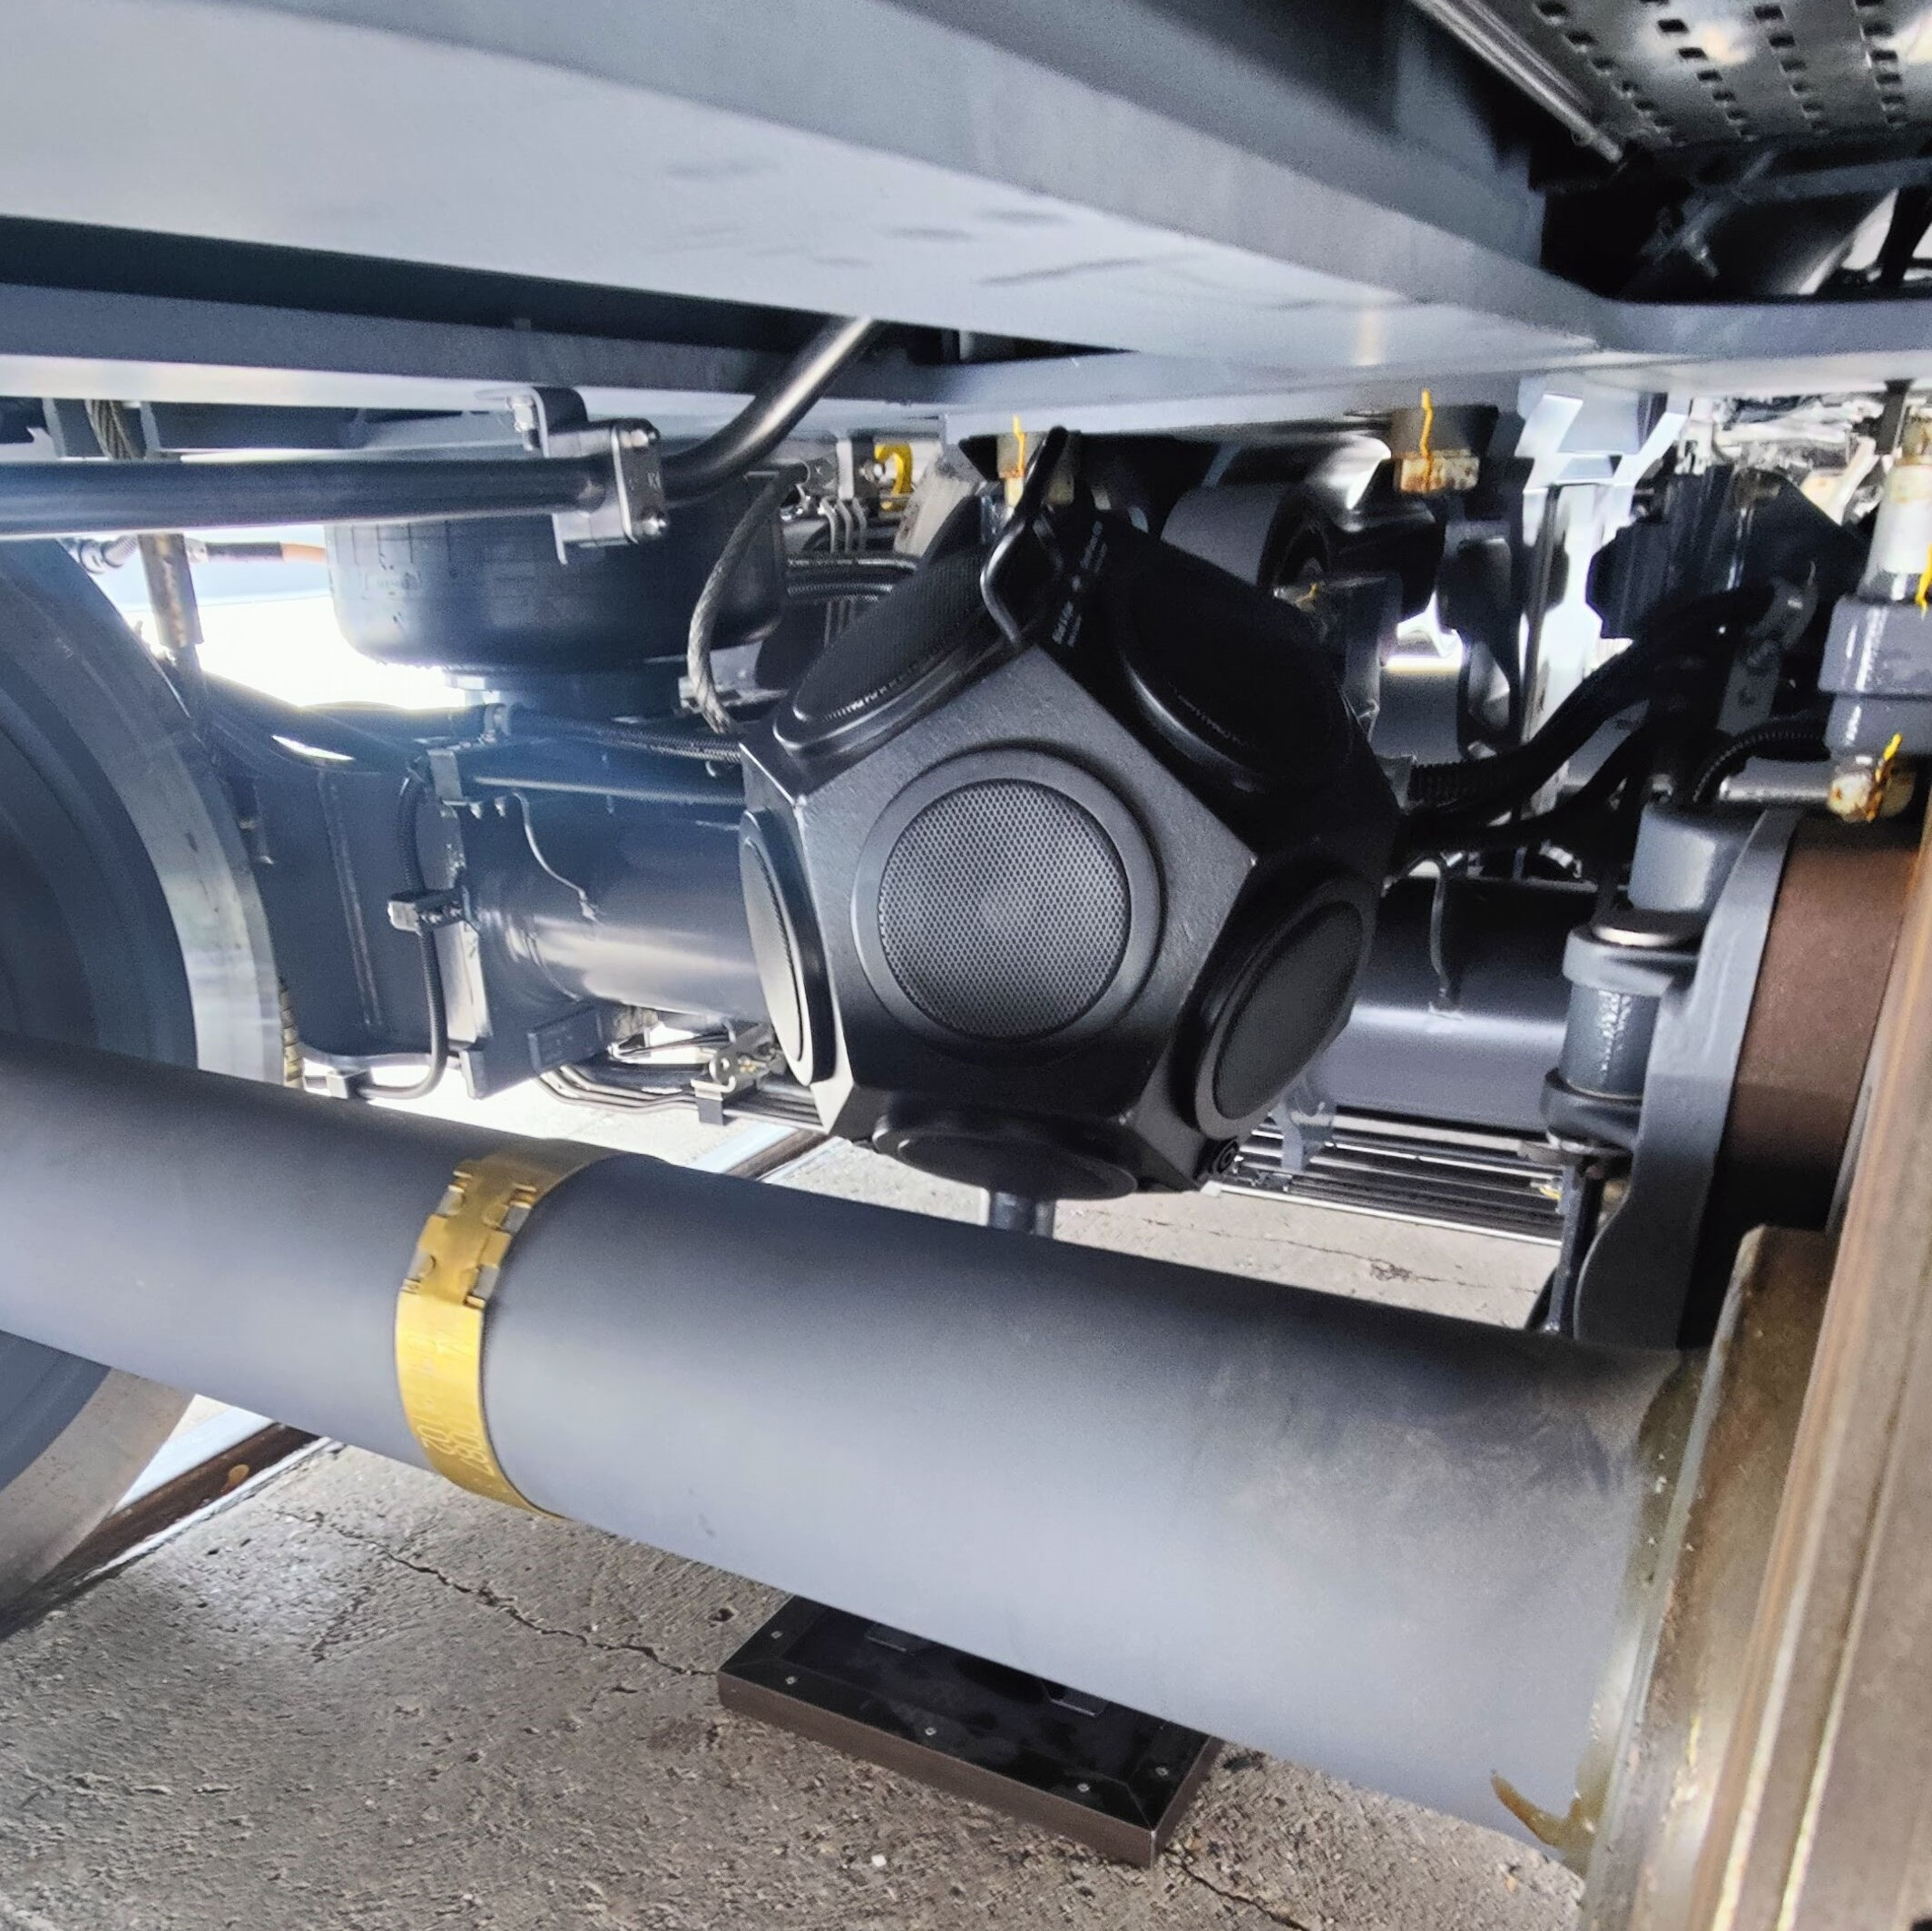
\includegraphics[width=\linewidth]{fig/loudspeaker_position_A.jpg}
         \caption{Position A: front of the bogie}
     \end{subfigure}
     %\par\bigskip
     \hspace{0.1\textwidth}
     %\hfill
     \begin{subfigure}[b]{0.4\textwidth}
         \centering
         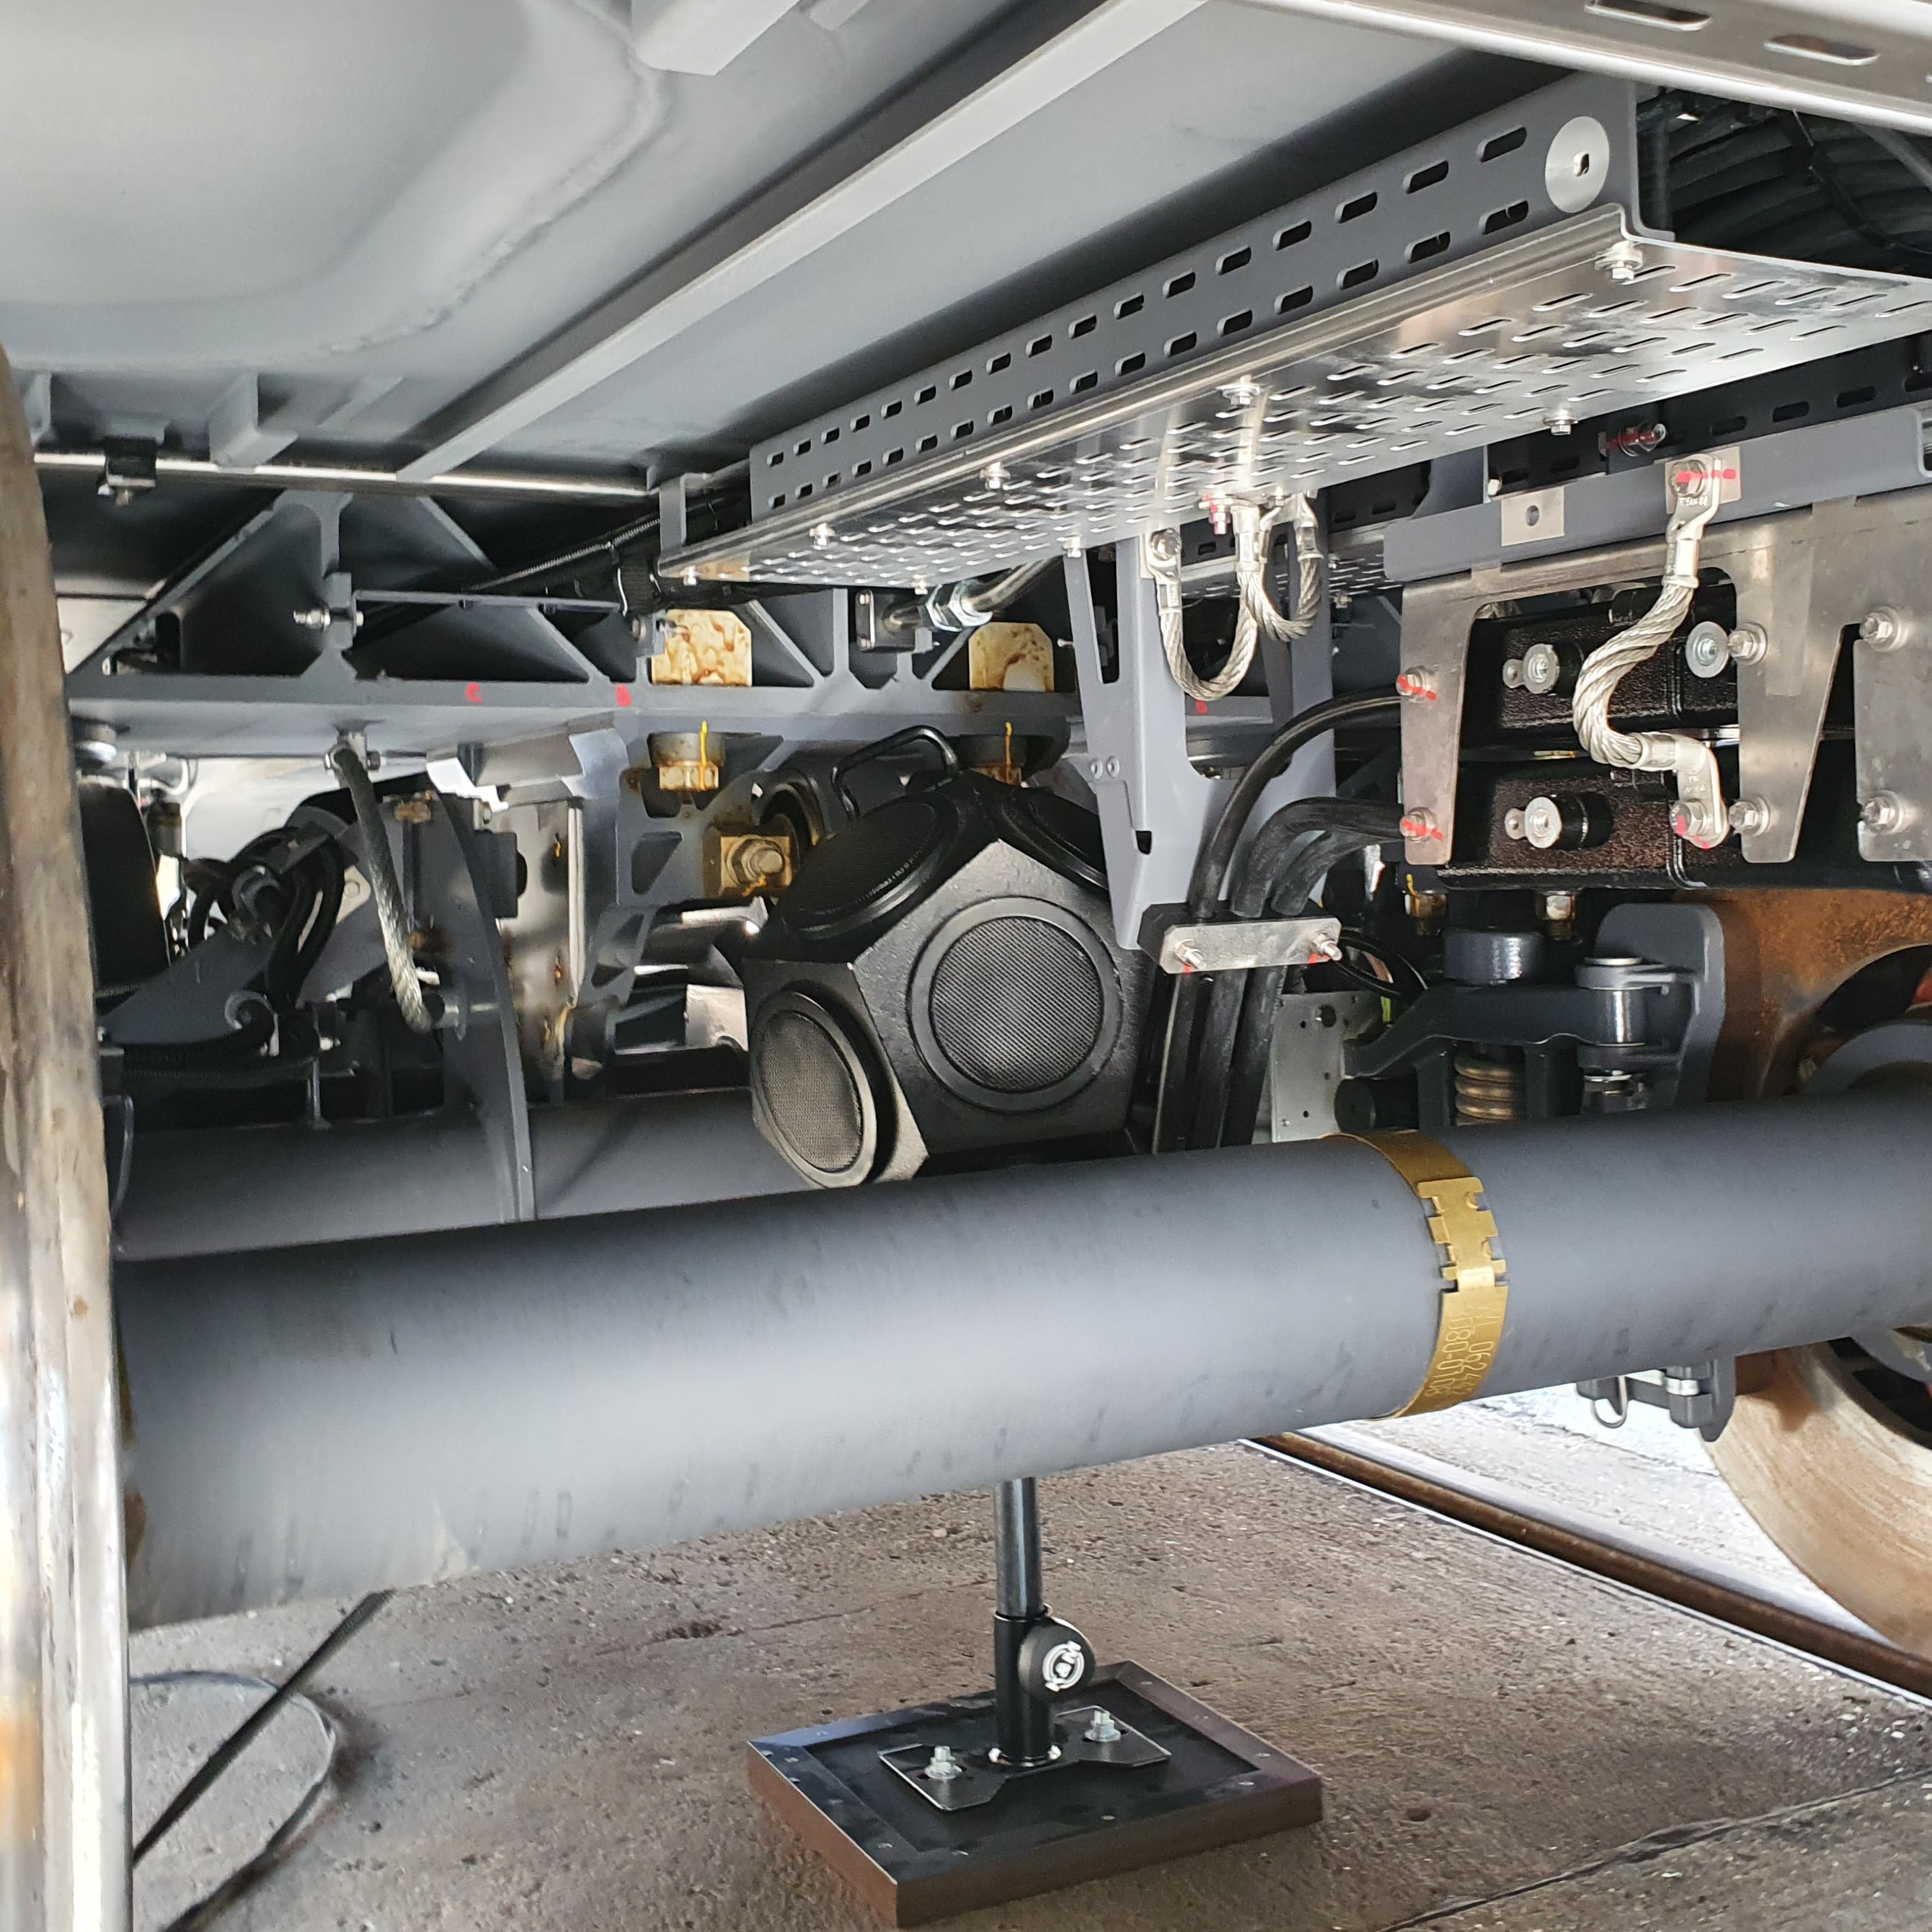
\includegraphics[width=\linewidth]{fig/loudspeaker_position_B.jpg}
         \caption{Postition B: rear of the bogie}
     \end{subfigure}
     \caption{Loudspeaker locations.}
     \label{fig:loudspeakerposition}
\end{figure}

\begin{figure}[H]
     \centering
     \begin{subfigure}[b]{\textwidth}
         \centering
         \includegraphics[width=\linewidth]{fig/Measurement_positions.png}
         \caption{Measurement positions a to i}
     \end{subfigure}
     %\par\bigskip
     %\hspace{0.1\textwidth}
     %\hfill
\end{figure}

\begin{figure}[H]\ContinuedFloat
    \centering
    \begin{subfigure}[b]{0.6\textwidth}
         \centering
         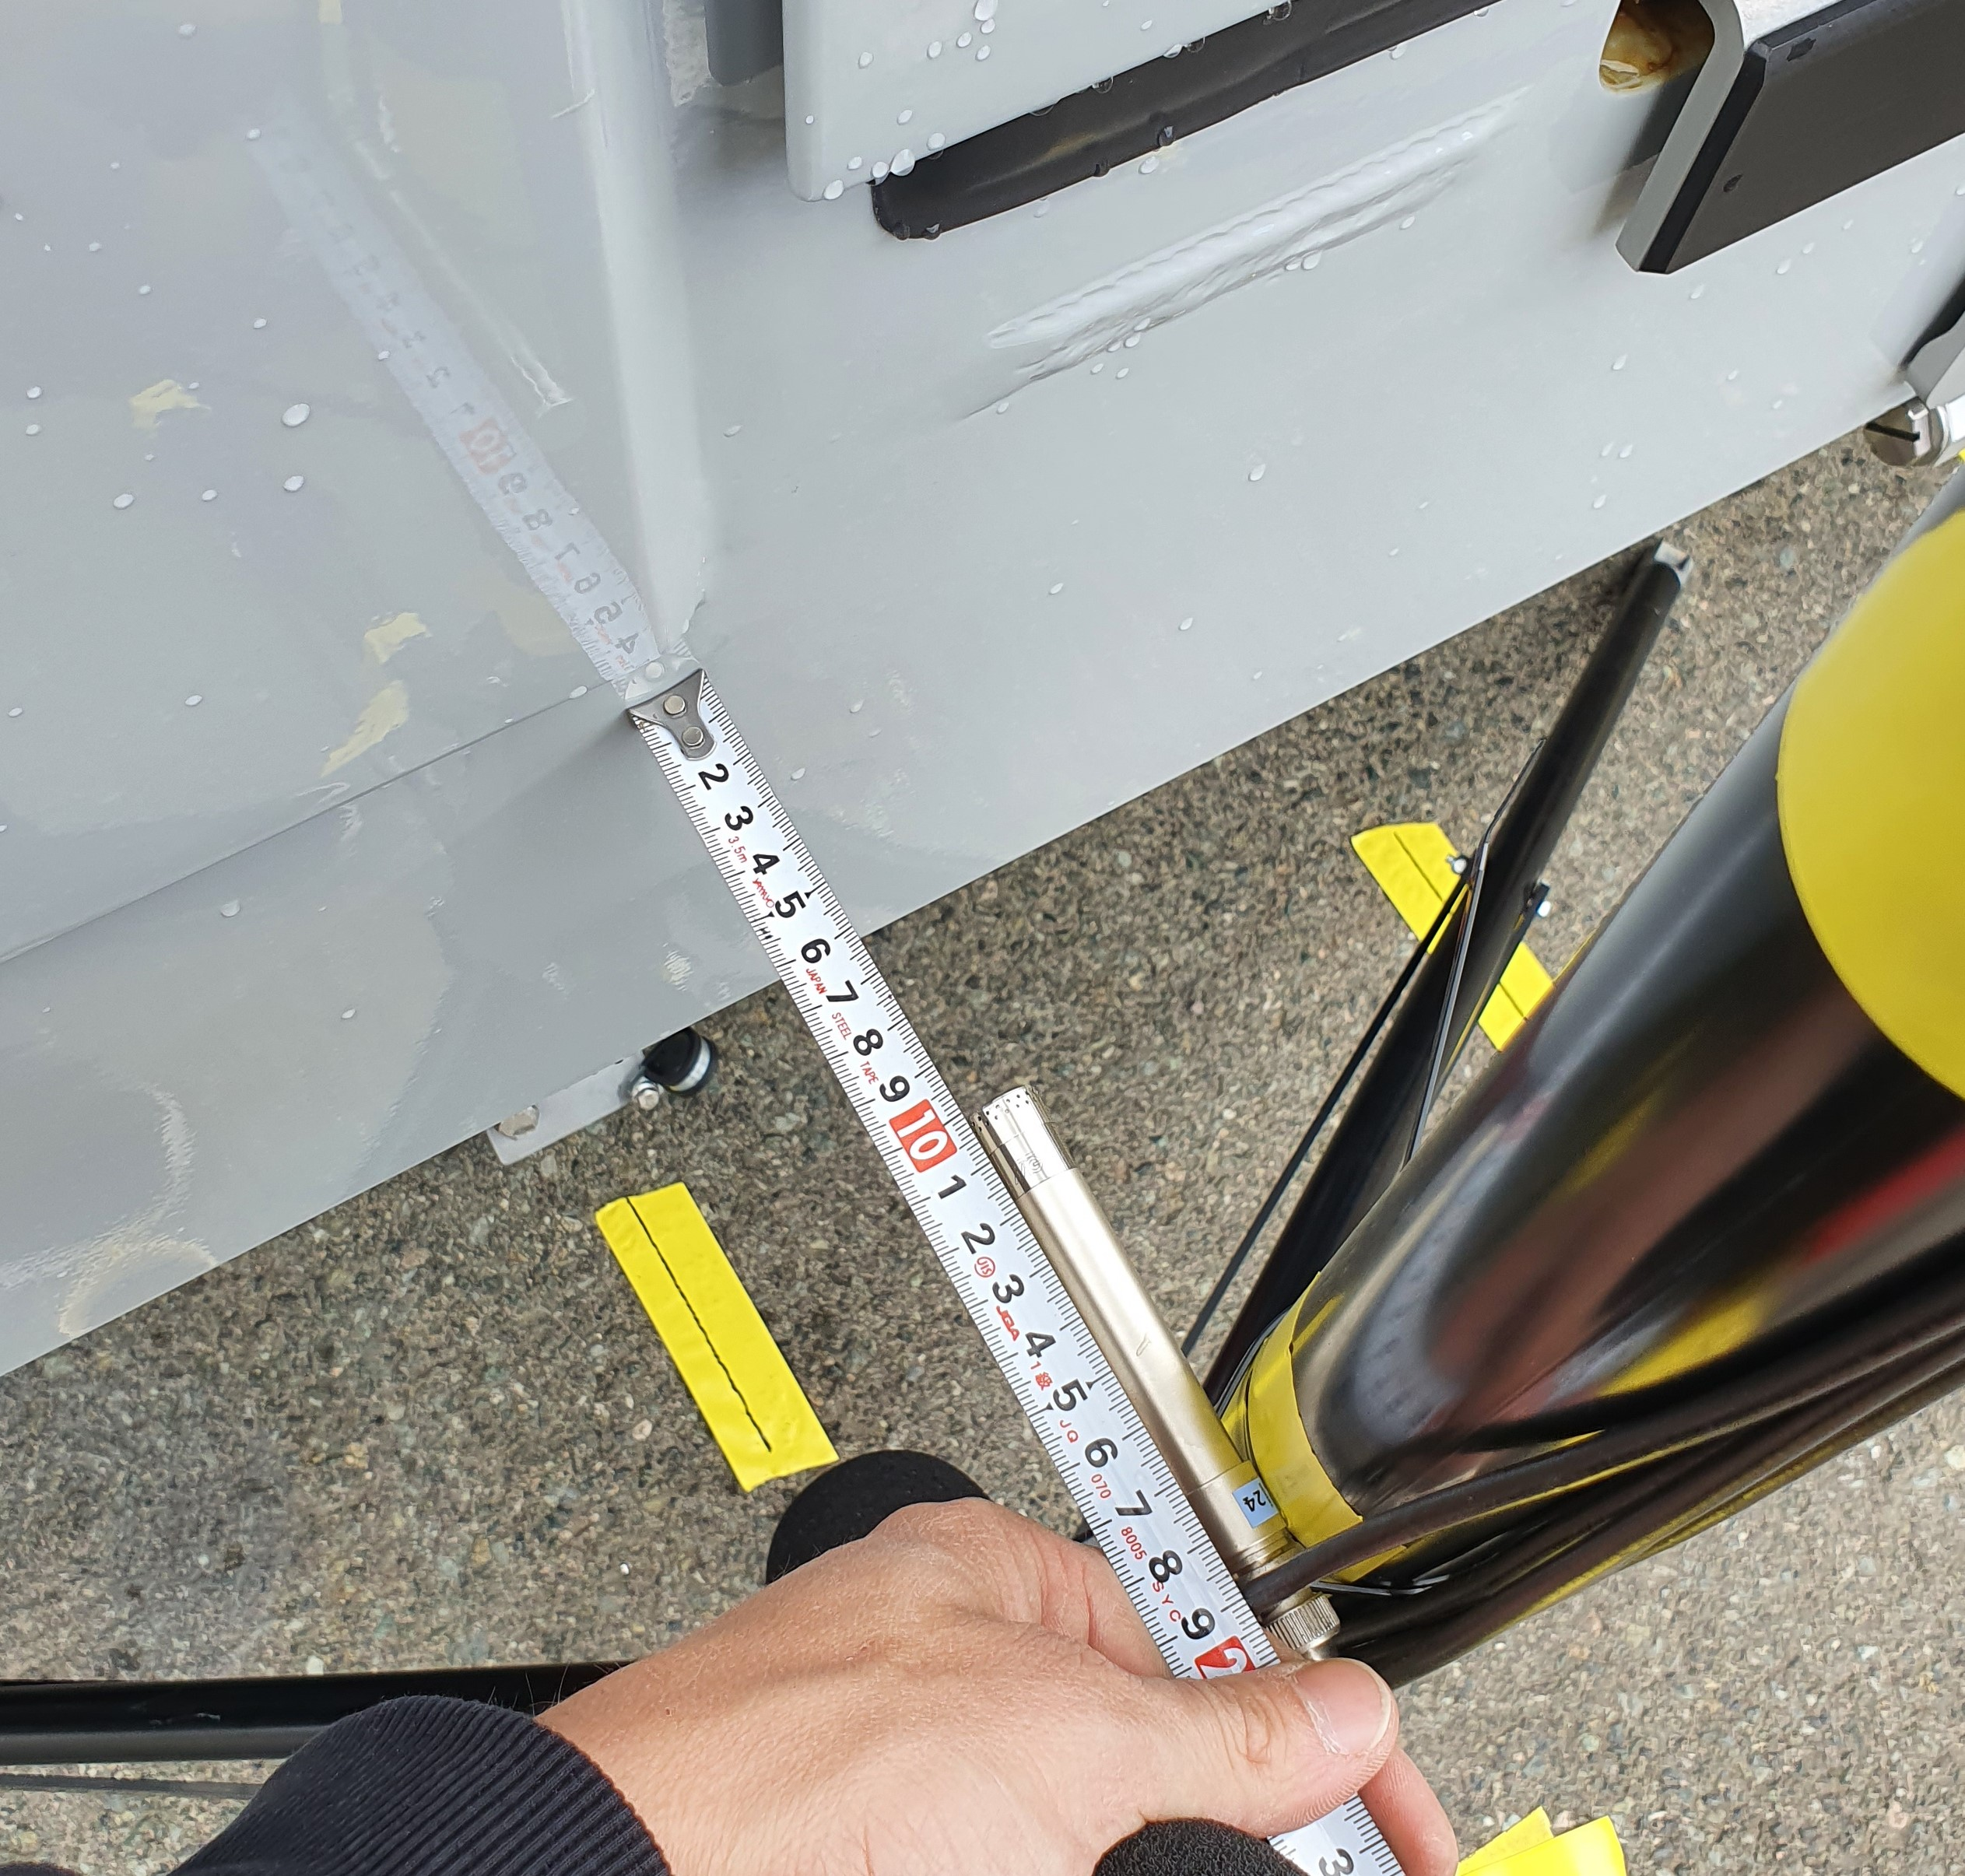
\includegraphics[width=\linewidth]{fig/position_of_microphones.jpg}
         \caption{Postition a: centerline of the bogie, 10 cm away from carbody edge}
         \label{fig:position_a}
     \end{subfigure}
     \caption{Measurement positions of microphone array.}
     \label{fig:microphoneposition}
\end{figure}

\subsection*{Measurement results}

In \cref{fig:timedomain}, the measured time signal of microphone 1 (0.5 m above ground) at measurment position a (front bogie centerline, 10 cm away from car body) with loudspeaker placed at the front of the bogie are shown. The signal was converted into frequency domain using fourier transformation as shown in \cref{fig:frequencydomain}. The post-processing was done directly in the provided software suit Müller-BBM PAK 6.x. \Cref{fig:fftparameter} shows a screenshot of the software GUI and the FFT parameters used are circled.

In \cref{fig:frequencydomain}, the blue curve shows the amplitude of acoustic pressure in narrow band resolution. The narrow band data was converted to 1/n octave form by summing up the amplitude of narrow-band spectral lines contained within the corresponding frequency bandwidth. The advantage of post-processing the data into octave bands is that it provides clearer information about the frequency composition of the noise signal. For example, it can be observed that in the 1/3 octave curve in \cref{fig:frequencydomain}, the peak of the SPL appears at 315 Hz, which also matches the peak in the SWL spectrum of the sound source as shown in \cref{fig:average_SWL}.

\begin{figure}[H]
    \centering
    \begin{subfigure}[b]{0.48\textwidth}
        \centering
        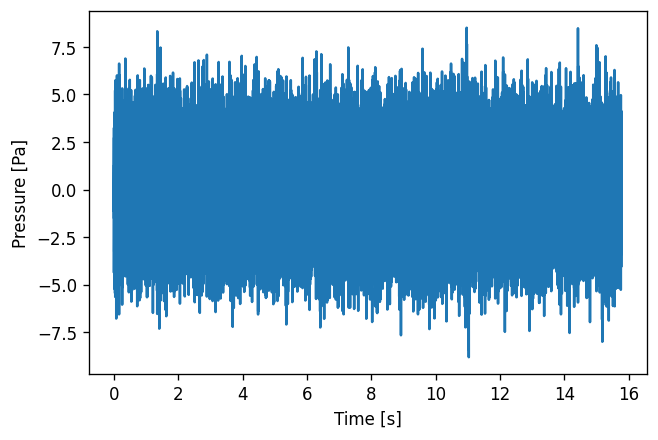
\includegraphics{fig/time_signal.png}
        \caption{Time domain}
        \label{fig:timedomain}
    \end{subfigure}
    \begin{subfigure}[b]{0.48\textwidth}
        \centering
        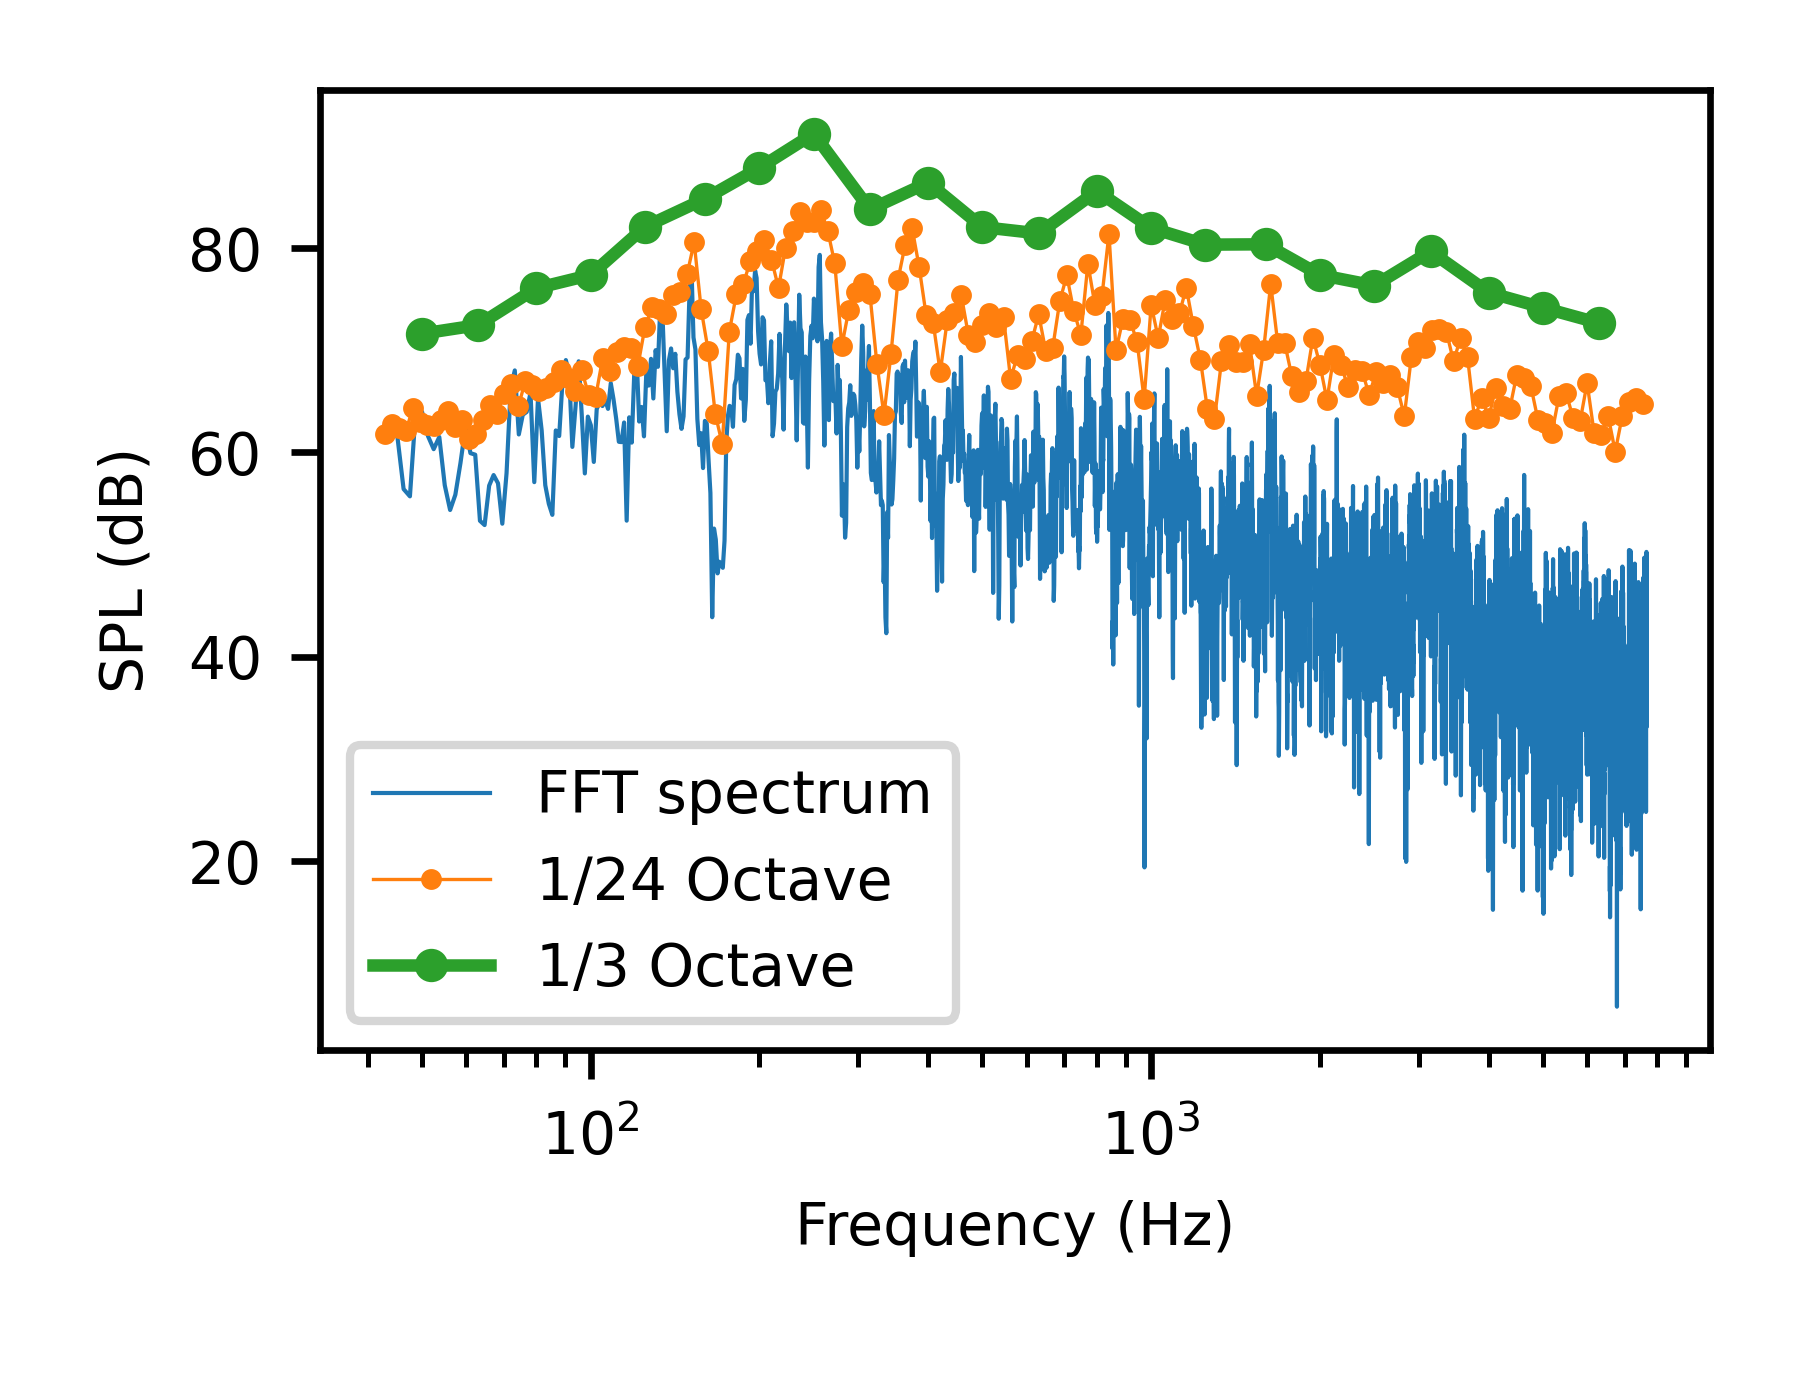
\includegraphics{fig/fft_spectra.png}
        \caption{Frequency domain}
        \label{fig:frequencydomain}
    \end{subfigure}
    
    \caption{Mesurement data at position a, microphone 1 (0.5 m), loudspeaker front.}
    \label{fig:measurementsignal}
\end{figure}

\begin{figure}[H]
    \centering
    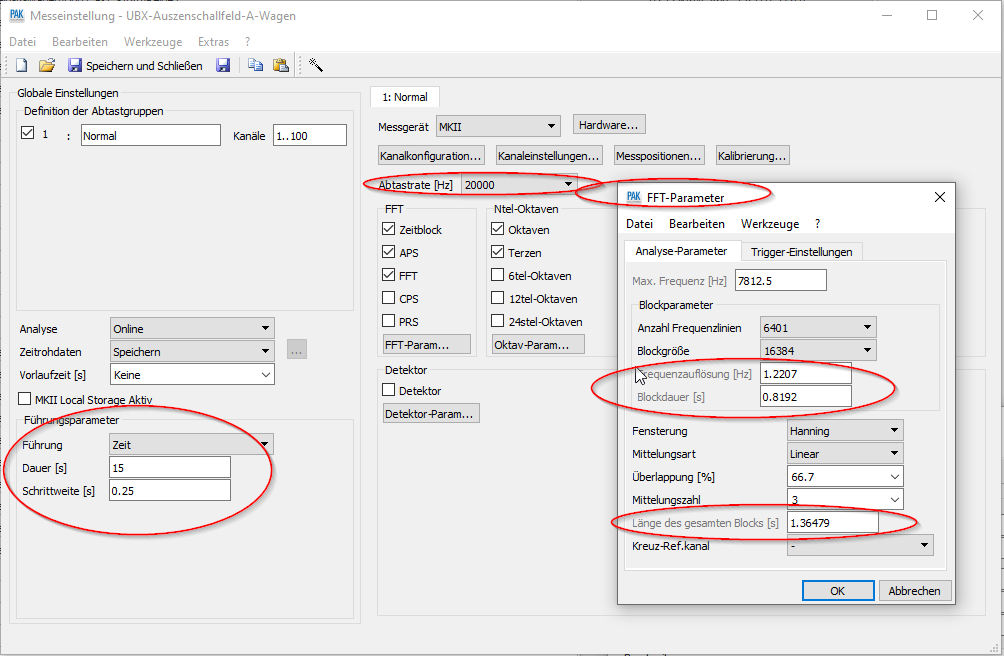
\includegraphics[width=\linewidth]{fig/fft_parameter.png}
    \caption{GUI of the Müller-BBM PAK software and FFT parameters used.}
    \label{fig:fftparameter}
\end{figure}

\begin{figure}[H]
    \centering
     \begin{subfigure}[b]{0.49\textwidth}
        \centering
        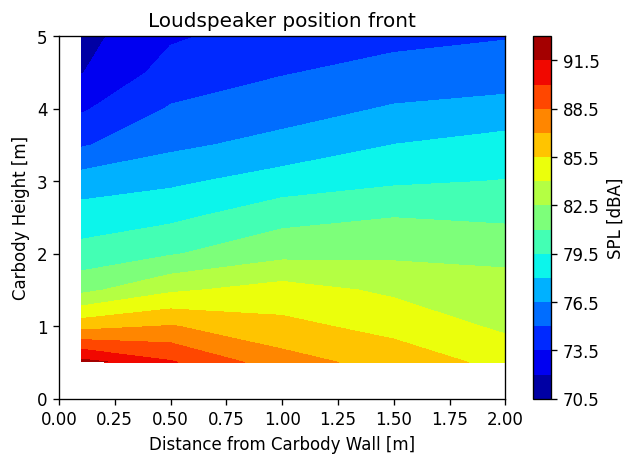
\includegraphics[width=\textwidth]{fig/pressure_field_loudspeaker_front.png}
        \caption{Loudspeaker position front}
    \end{subfigure}
    \begin{subfigure}[b]{0.49\textwidth}
        \centering
        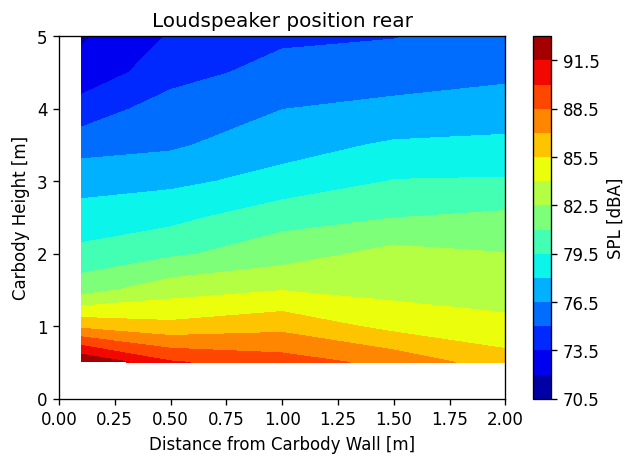
\includegraphics[width=\textwidth]{fig/pressure_field_loudspeaker_rear.png}
        \caption{Loudspeaker position rear}
    \end{subfigure}
        \caption{Pressure field around car body.}
        \label{fig:pressurefield}
\end{figure}

\noindent In \cref{fig:pressurefield}, a visualization of the total pressure field around the car body is shown. The horizontal axis represents the distance from car body wall, the vertical axis the height above ground and the color the overall A-weighted pressure level, respectively. The white space in the plot is due to the missing data in the measurement since the measurement positions start at 10 cm away from car body wall and half meter above ground. Comparing the pressure field of the two different loudspeaker locations, the asymmetric effect introduced by the brake disc can be observed. The brake disc of the front wheel axle standing in the transmission path of the loudspeaker seems to block a part of the acoustic wave.

\begin{figure}[H]
    \centering
     \begin{subfigure}[b]{0.48\textwidth}
        \centering
        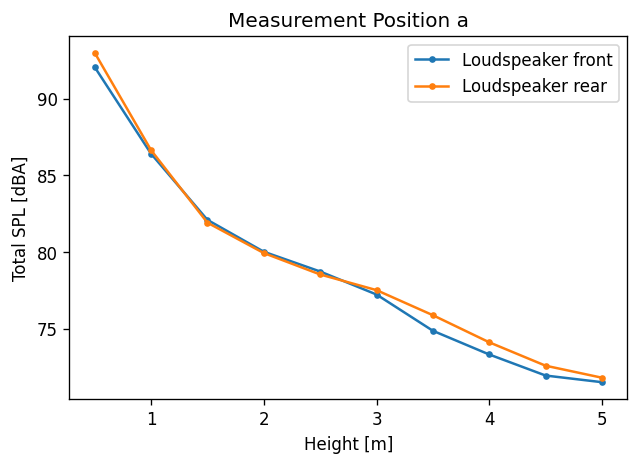
\includegraphics{fig/pressure_over_height_pos_a.png}
        \caption{Measurement position a}
        \label{fig:SPLoverheight_pos_a}
    \end{subfigure}
    \begin{subfigure}[b]{0.48\textwidth}
        \centering
        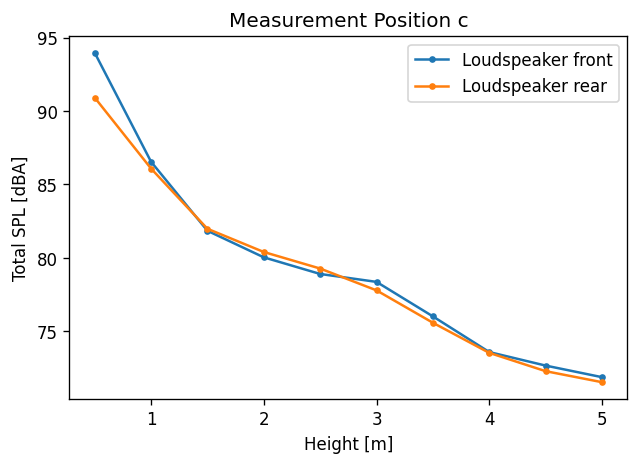
\includegraphics{fig/pressure_over_height_pos_c.png}
        \caption{Measurement position c}
        %\label{fig:frequencydomain}
    \end{subfigure}
    \caption{Overall A-weighted sound pressure level at example measurement positions.}
    \label{fig:SPLoverheight}
\end{figure}

\noindent In order to compare the pressure field quantitatively, one can plot the acoustic pressure as function of height for different measurement positions, which can be seen in the figures above. In \ref{fig:SPLoverheight_pos_a} it can be observed that at measurement position a, the pressure curve caused by loudspeaker at different locations shares similar shape, and the pressure is strictly decreasing over carbody height.

\begin{figure}[H]
    \centering
     \begin{subfigure}[b]{0.48\textwidth}
        \centering
        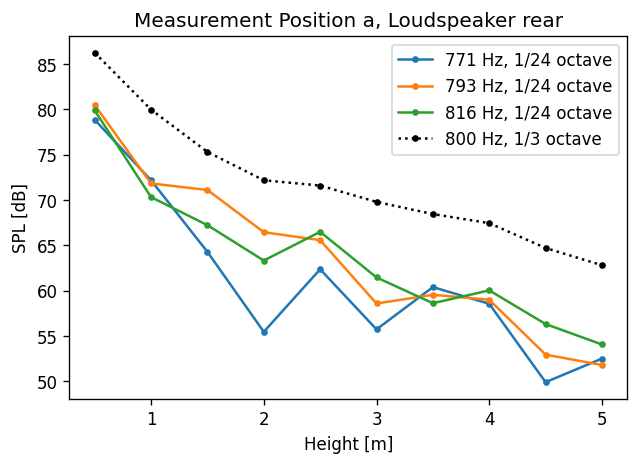
\includegraphics{fig/pressure_over_height_800Hz.png}
        \caption{800 Hz}
        \label{fig:SPLoverheight_frequency_800Hz}
    \end{subfigure}
    \begin{subfigure}[b]{0.48\textwidth}
        \centering
        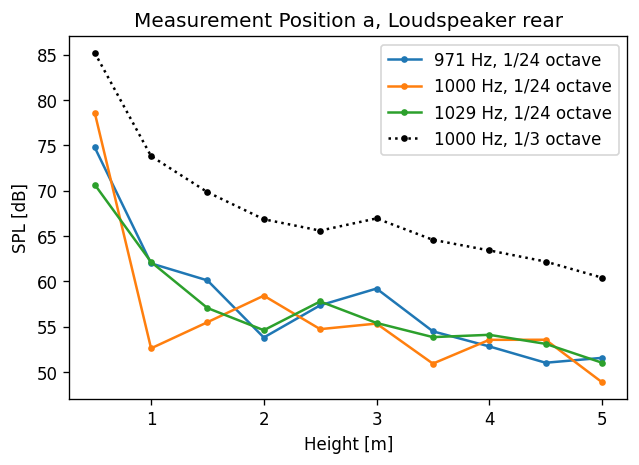
\includegraphics{fig/pressure_over_height_1000Hz.png}
        \caption{1000 Hz}
        \label{fig:SPLoverheight_frequency_1000Hz}
    \end{subfigure}
    \caption{SPL distribution of example third octave bands at measurement position a with loudspeaker at the rear. Solid line: 1/24-octave center frequency. Dashed line: 1/3-octave center frequency.}
    \label{fig:SPLoverheight_frequency}
\end{figure}

\noindent In fig. \ref{fig:SPLoverheight_frequency}, the sound pressure level over height for different 1/n octave band center frequencies is displayed. In the 1/24 octave resolution, several local minima in the curve shape can be observed, e.g. for 771 Hz in fig. \ref{fig:SPLoverheight_frequency_800Hz} or for 1000 Hz in fig. \ref{fig:SPLoverheight_frequency_1000Hz}, which are caused by the destructive interference of the acoustic wave. The destructive interference can also be observed in the pressure field of the single frequency band as shown in fig. \ref{fig:pressurefield_1000Hz}, sinks in acoustic field are to be found at about 1 m and 3.5 m height, respectively, which correspond to the position of the local minima in fig. \ref{fig:SPLoverheight_frequency_1000Hz}.

\begin{figure}[H]
    \centering
    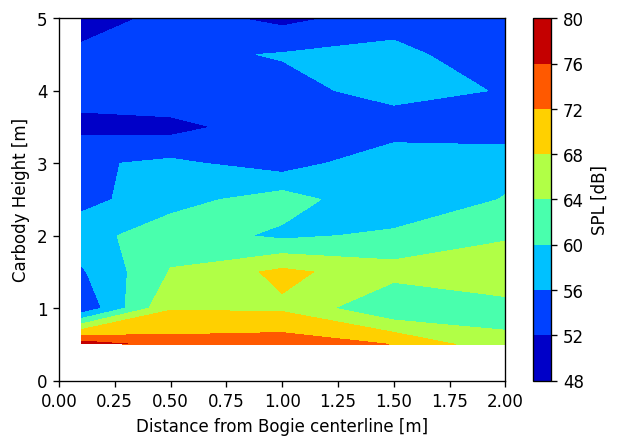
\includegraphics[width=0.6\linewidth]{fig/pressure_field_1000Hz.png}
    \caption{Pressure field of 1/24-octave frequency 1000 Hz with loudspeaker placed at the rear.}
    \label{fig:pressurefield_1000Hz}
\end{figure}
